\section{Problem Set 1}
\subsection{Your Mission, Your Challenge}

We conducted an in-depth survey of existing and proposed Distributed Space Systems, and decided on a fictional concept consisting of a swarm performing in-orbit servicing. We are calling this fictional mission SOSS: Servicing and Observing Satellite Swarm. The goal of the mission is to have two unique satellites observe and operate on an existing satellite (called the \textbf{Target}) that needs to be serviced. The two satellites in the mission are called the \textbf{Watcher} and the \textbf{Docker}. The Watcher's objective is to observe the other two satellites and provide relative navigation information. The Docker's objective is to rendezvous with the Target and provide services such as in-space refueling and robotic servicing.

We are using Starling \cite{krugerorbit} as a baseline for numerical values for initial orbital configurations, and for swarm behavior in future assignments. We are also interested in the application of relative optical navigation, demonstrated by Starling, for our mission.

\subsubsection{Mission Name and Operator}
We are designing a mission called \textbf{SOSS}: \textbf{S}ervicing and \textbf{O}bserving \textbf{S}atellite \textbf{S}warm. Operated by the Chigullapalli-Bogdanowitsch Space Agency (CBSA)

\subsubsection{Primary and Secondary Mission Objectives}
\begin{itemize}
    \item Primary objective is to service and extend the mission lifetime of an existing Target satellite.
    \item Secondary objective is to demonstrate in-orbit visual navigation for spacecraft rendezvous.
\end{itemize}
    
\subsubsection{Number and Type of Satellites}
3 satellites in the swarm. SV1 is the Target, and is the satellite we are servicing. SV2 is the Watcher, equipped with vision sensors. SV3 is the Docker, responsible for docking and equipped with servicing equipment (robotic arm, propellant tanks).

\subsubsection{Absolute Orbit Parameters}
Inherited from the Starling mission \cite{krugerorbit}, the quasi-nonsingular absolute orbit parameters of SV4 of the Starling swarm are as follows:
\begin{table}[h]
\centering
\begin{tabular}{cccccc} \hline
    $a$ & $e_x$ & $e_y$ & $i$ & $\Omega$ & $u$ \\ \hline 
     6944 km & -0.00004 & 0.0016 & 99.4 $^\circ$ & -151.1$^\circ$ & -47.9$^\circ$ \\ \hline
\end{tabular}
\caption{Absolute Orbit Parameters}
\label{tab:abs_oe}
\end{table}

We will take these parameters to be our Target SV1. 

The quasi-nonsingular absolute orbit is given by D'Amico \cite{damicothesis} as:
\begin{align}
\boldsymbol{\alpha} &= 
\begin{bmatrix}
a & e_x & e_y & i & \Omega & u
\end{bmatrix}^\top \notag \\
&= 
\begin{bmatrix}
a & e \cos \omega & e \sin \omega & i & \Omega & \omega + M
\end{bmatrix}^\top \tag{3}
\end{align}

where $a, e, i, \Omega, \omega, M$ are the Keplerian orbit elements. These are converted to standard Keplerian orbital elements in Section \ref{sec:initial_oe}.

\subsubsection{Relative Orbit Parameters}\label{sec:ROE_init}
Again, inheriting from the Starling mission, the quasi-nonsingular relative orbit elements (ROE) of SV3 and SV2 with respect to SV4 are given by the following. These parameters, along with the absolute ones, occurred at 02/05/24 00:00:00 UTC, but we will define them as our starting parameters at an arbitrary point in the future: 
\begin{table}[h!]
\centering
\begin{tabular}{ll}
\toprule
\textbf{ID} & \textbf{In-Train Formation} \\
\midrule
SV2 & $\delta\boldsymbol{\alpha} = [21, -124350, 110, 202, 79, 1005]~\text{m}$ \\
SV3 & $\delta\boldsymbol{\alpha} = [-1, -79328, 42, 452, 36, 827]~\text{m}$ \\
\bottomrule
\end{tabular}
\end{table}

We will take the Starling SV4 to be our Target SV1, the Starling SV2 to be our Watcher SV2, and Starling SV3 to be our Docker SV3. 

The quasi-nonsingular ROE adopted by D'Amico \cite{damicothesis} are a function of the orbit elements of the target $t$ and observer $o$. They are given by:
\begin{align}
\delta \boldsymbol{\alpha} &= 
\begin{bmatrix}
\delta a & \delta \lambda & \delta e_x & \delta e_y & \delta i_x & \delta i_y
\end{bmatrix}^\top \notag \\
&= 
\left( 
\begin{bmatrix}
\delta a \\
\delta \lambda \\
|\delta\mathbf{e}| \cos \phi \\
|\delta\mathbf{e}| \sin \phi \\
|\delta\mathbf{i}| \cos \theta \\
|\delta\mathbf{i}| \sin \theta
\end{bmatrix}
= 
\begin{bmatrix}
\frac{a_t - a_o}{a_o} \\
(u_t - u_o) + (\Omega_t - \Omega_o) \cos i_o \\
e_{x,t} - e_{x,o} \\
e_{y,t} - e_{y,o} \\
i_t - i_o \\
(\Omega_t - \Omega_o) \sin i_o
\end{bmatrix}
\right) \tag{4}
\end{align}

where $[\delta e_x, \delta e_y]$ are components of the relative eccentricity vector with phase $\phi$ and $[\delta i_x, \delta i_y]$ are components of the relative inclination vector with phase $\theta$.    

\subsubsection{Launch Date and Mission Duration} 
May 8th, 2031; 6 month mission duration.

\subsubsection{Key DGN\&C requirements}


The swarm and rendezvous requirements for the Watcher, Docker, and the relation between those satellites and the Target are given as (and inspired again by the requirements for the Starling mission \cite{kruger2024starling}):

\begin{itemize}
    \item The inter-satellite distance between the Watcher and the Docker shall not exceed the limit for inter-satellite communication.
    \item The Watcher shall have the Target in its camera's field of view at all times 
    \item The Watcher shall maintain a safe inter-satellite distance to the Docker and Target, on the order of $\approx100$ meters, at all times.
    \item The Watcher's bearing angle measurements of the Target/Docker shall not remain constant.
    \item When not in the final docking phase, the Docker shall maintain a safe inter-satellite distance to the Target on the order of $\approx 100$ meters.
    \item During the docking phase, the Docker shall compute a fuel-optimal rendezvous trajectory to the Target.
    \item The Docker shall track the optimal rendezvous trajectory to $\approx 10 cm$ accuracy when in close-proximity to the Target.
    \item The Watcher shall provide a relative position measurement of the Docker/Target around the $\approx 10 cm$ accuracy.
    \item During the docking phase, the Watcher shall have both the Target and Docker in its camera's field of view.
    \item All satellites shall stay in a stable low-earth orbit for the entirety of the mission.
\end{itemize}


\subsubsection{Classification of DSS} 
Our mission will be a Swarm that involves Rendezvous and Docking. We classify this mission as a swarm based on the small inter-satellite separation when orbiting close to the Target satellite and the high navigation accuracy required in such a situation. The mission is also a Rendezvous and Docking mission because the requirements have the Docker and Target docking.

\subsection{Orbit Simulation, Review of Astrodynamics}
\subsubsection{Initial Orbital Elements} \label{sec:initial_oe}
The initial conditions are taken from the Starling mission literature \cite{krugerorbit} and are provided in Table \ref{tab:abs_oe}. These elements, originally provided in the quasi-nonsingular absolute orbit parameters, were first converted to the Keplerian orbital elements, which are given in Table \ref{tab:abs_oe_kepler}.

\begin{table}[h]
\centering
\begin{tabular}{cccccc} \hline
    $a$ & $e$ & $i$ & $\omega$ & $\Omega$ & $\nu$ \\ \hline 
     6944 km & 0.0016 & 99.4 $^\circ$ & 91.432$^\circ$ & -151.1$^\circ$ & -139.45$^\circ$ \\ \hline
\end{tabular}
\caption{Inital Keplerian Orbit Parameters of SV1}
\label{tab:abs_oe_kepler}
\end{table}

For future use, it is also useful to note that the corresponding initial mean anomaly $M_0= -139.33^\circ$.

The quasi-nonsingular absolute orbit parameters were converted to the Keplerian orbital elements by using the following procedure. First, compute the argument of perigee, eccentricity, and the mean anomaly:
\[
\omega = \tan^{-1} \left( \frac{e_y}{e_x} \right)
\]
\[
e = \frac{e_x}{\cos \omega}
\]
\[
M = u - \omega
\]

Then, convert mean anomaly to radians and solve Kepler's equation using Newton-Raphson to obtain eccentric anomaly \( E \).

Finally, compute the true anomaly:
\[
\nu = \tan^{-1} \left( \frac{\sqrt{1 + e} \cdot \tan(E/2)}{\sqrt{1 - e}} \right) \cdot 2
\]

\subsubsection{Initial Position and Velocity in ECI}\label{sec:initial_ECI}
 Treating the initial Keplerian orbital elements for the target SV1 given in Table \ref{tab:abs_oe_kepler} as osculating quantities, they can be converted into Earth-Centered Inertial (ECI) position (in km) and velocity (in km/s), and are 
 \begin{align}
     \boldsymbol{r}_{0, ECI, SV1} &= \begin{bmatrix}
         -3663.3 \\
         -2986.4 \\
         -5098.8
     \end{bmatrix} \\
     \boldsymbol{v}_{0, ECI, SV1} &= \begin{bmatrix}
         -5.3201 \\
         -1.9915 \\
         4.9994
     \end{bmatrix}.
 \end{align}

The conversion from Keplerian orbital elements to ECI position and velocity is as follows. First, we calculate norm of the position $r$:

\[
r = \frac{a(1 - e^2)}{1 + e \cos \nu}
\]

And then transform it into the PQW (perifocal) frame:
\[
\mathbf{r}_{PQW} = \begin{bmatrix}
r \cos \nu \\
r \sin \nu \\
0
\end{bmatrix}
\]

Next we compute mean motion:
\[
n = \sqrt{\frac{\mu}{a^3}}
\]

And then we compute the eccentric anomaly:
\[
E = 2 \cdot \tan^{-1} \left( \sqrt{\frac{1 - e}{1 + e}} \cdot \tan\left(\frac{\nu}{2}\right) \right)
\]

The rotation matrix from PQW to ECI (IJK) frame is given by:
\[
R_{\text{PQW} \to \text{ECI}} = 
\begin{bmatrix}
\cos\Omega\cos\omega - \sin\Omega\cos i\sin\omega & -\cos\Omega\sin\omega - \sin\Omega\cos i\cos\omega & \sin\Omega\sin i \\
\sin\Omega\cos\omega + \cos\Omega\cos i\sin\omega & -\sin\Omega\sin\omega + \cos\Omega\cos i\cos\omega & -\cos\Omega\sin i \\
\sin i\sin\omega & \sin i\cos\omega & \cos i
\end{bmatrix}
\]

And the velocity in PQW frame is:
\[
\mathbf{v}_{PQW} = \frac{a n}{1 - e \cos E}
\begin{bmatrix}
-\sin E \\
\sqrt{1 - e^2} \cos E \\
0
\end{bmatrix}
\]

Finally, we can transform to the ECI frame:
\[
\mathbf{r}_{ECI} = R_{\text{PQW} \to \text{ECI}} \cdot \mathbf{r}_{PQW}
\qquad
\mathbf{v}_{ECI} = R_{\text{PQW} \to \text{ECI}} \cdot \mathbf{v}_{PQW}
\]

\subsubsection{Numerical Simulation of State with Perturbations}
The state of the satellite is represented by 
\begin{align}
    \boldsymbol{x} = \begin{bmatrix}
        \boldsymbol{r}^T & \boldsymbol{v}^T
    \end{bmatrix}^T
\end{align}

The derivative of this state is given by 
\begin{align}
    \boldsymbol{\dot{x}} = \begin{bmatrix}
        \boldsymbol{v}^T & \boldsymbol{a}^T
    \end{bmatrix}^T
\end{align}

where $a$ is the acceleration on the satellite from the primary attractor. The acceleration due to gravity is given by
\begin{align}
    \boldsymbol{a_g} = \frac{-\mu}{||\boldsymbol{r}||^3} \boldsymbol{r}.
\end{align}

The additional J2 perturbation acceleration vector is given by 

\[
\mathbf{a}_{J2} = \frac{3 J_2 \mu R_e^2}{2 r^5} \begin{bmatrix}
\left(5\frac{r_z^2}{r^2} - 1\right) r_x \\
\left(5\frac{r_z^2}{r^2} - 1\right) r_y \\
\left(5\frac{r_z^2}{r^2} - 3\right) r_z
\end{bmatrix}
\]

Then the total acceleration when including J2 is

\[
\mathbf{a} = \mathbf{a}_{\text{g}} + \mathbf{a}_{J2}
\]

With these acceleration terms, we can propagate the state through an integer number of orbits (20 in our case) and obtain the orbital path. We used a custom Runge-Kutta (RK4) integrator with a fixed step size of $\frac{1}{500}$ of the orbit period to ensure accuracy. 

Figure \ref{fig:3d_plots_with_j2} shows the 3D plot of the orbit in an inertial frame, and compares the orbit with and without J2 perturbations.

\begin{figure}[H]
    \centering
    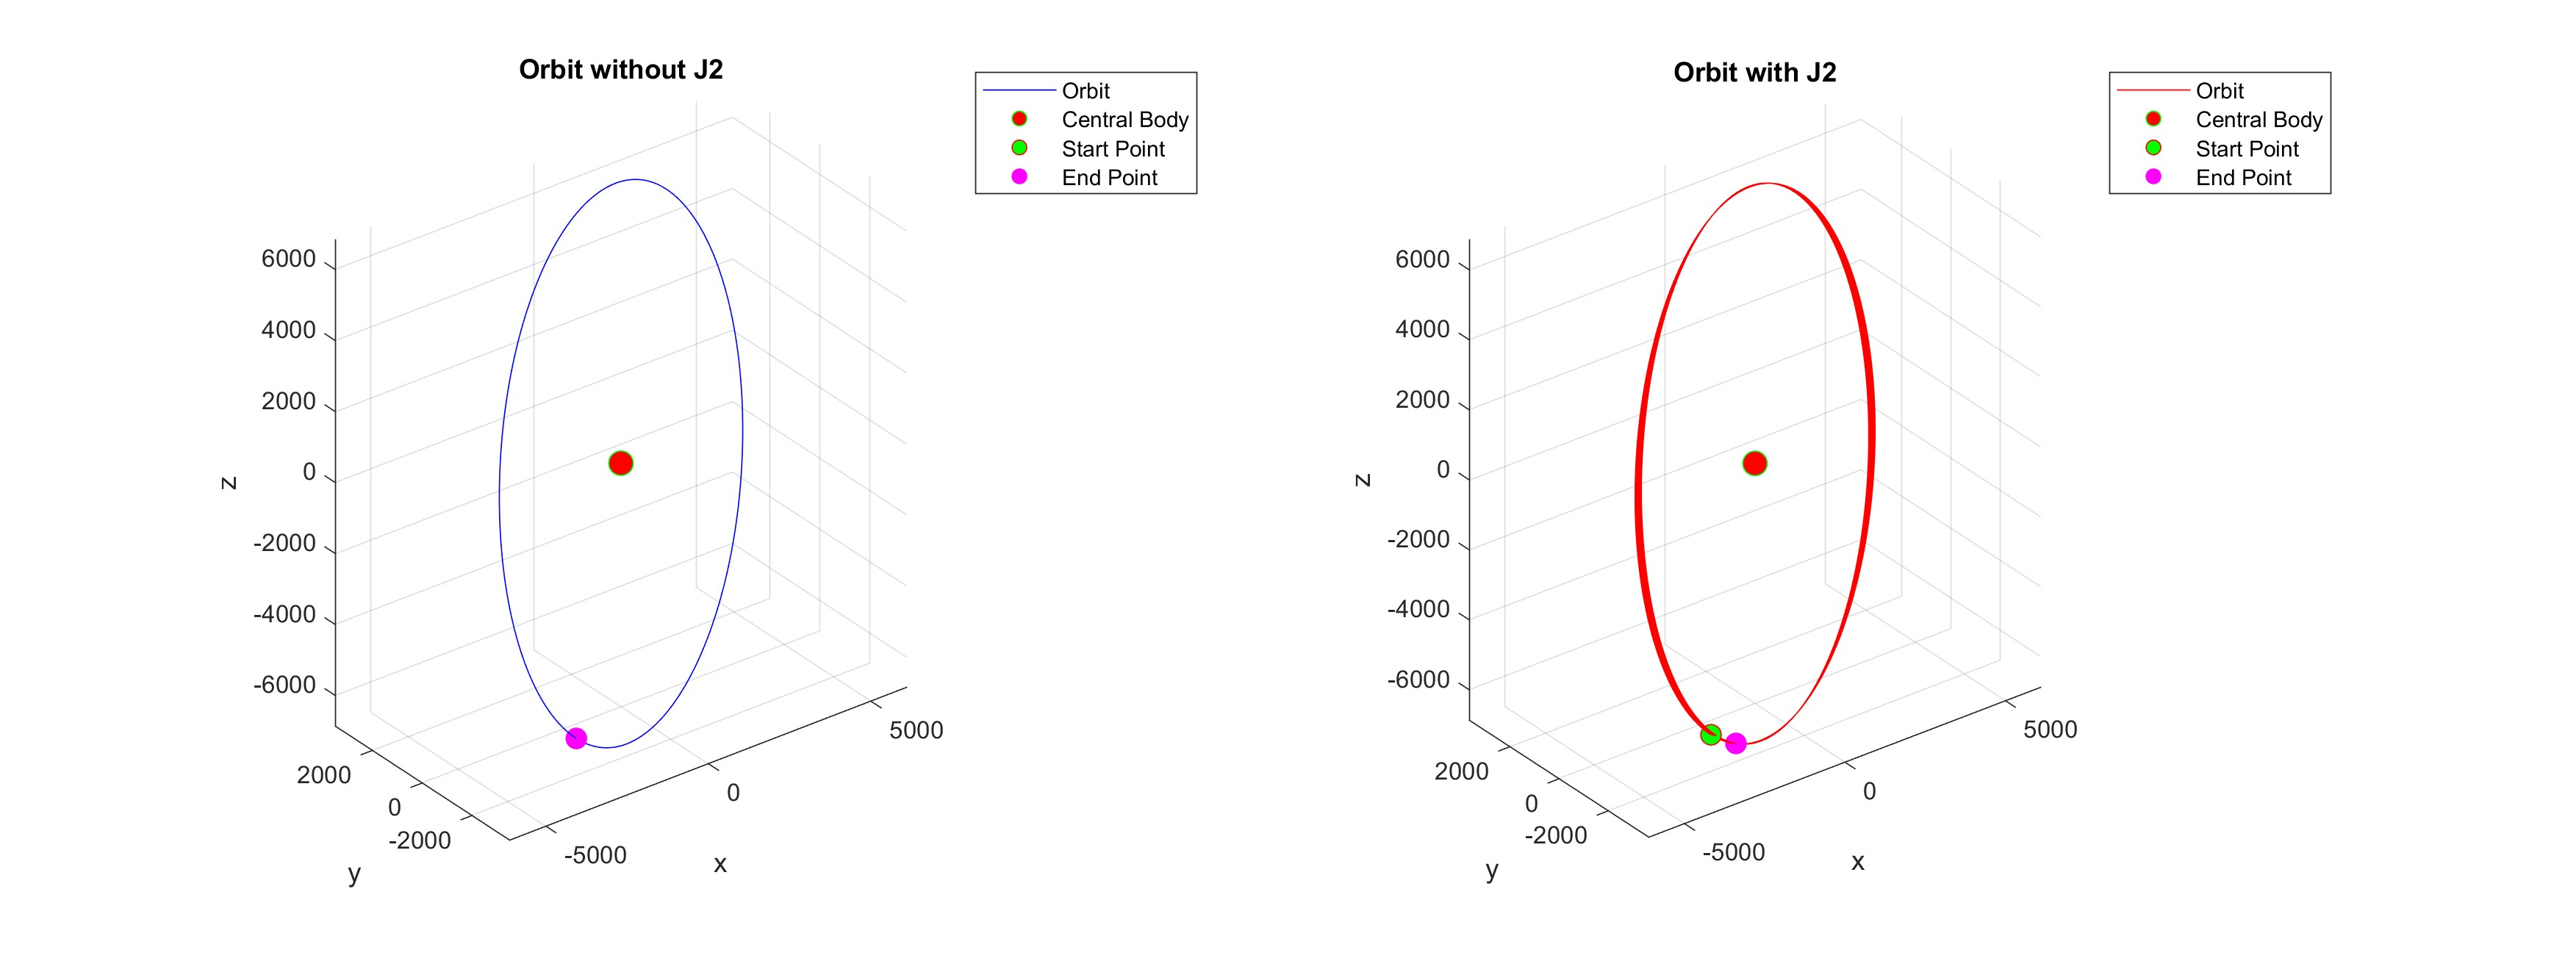
\includegraphics[width=1.1\linewidth]{PS1/Figures/Orbit_J2_Comparison_ECI.jpg}
    \caption{Comparison of the 3D plots with (right) and without (left) J2 perturbations. }
    \label{fig:3d_plots_with_j2}
\end{figure}

As expected, the most prominent change in the orbit with J2 perturbations is in the RAAN. The change in RAAN is secular rather than periodic, as will be seen in more detail in the plots in Section \ref{sec:oe_compares}.

\subsubsection{Comparison with Analytical Keplerian Propagation} \label{sec:analytical_and_eci2rtn}

We can compare the no-J2 simulation with the analytical Keplerian result for the orbital parameters mentioned in Table \ref{tab:abs_oe_kepler}, but by varying the true anomaly $\nu$. 

The time-steps used in the numerical propagation $t$ are converted into $\nu$ values (via intermediate computation of mean anomaly $M$ and eccentric anomaly $E$). The state outputs from both the numerical simulation and the analytical keplerian solution are converted from the ECI frame into the Radial-Tangent-Normal (RTN) frame.

The rotation matrix from ECI to RTN is done as follows:

\begin{align}
    \hat{R} &= \frac{r_{ECI}}{||r_{ECI}||} \\
    \hat{N} &= \frac{r_{ECI} \times v_{ECI}}{||r_{ECI} \times v_{ECI}||} \\
    \hat{T} &= \hat{N} \times \hat{R} \\
    Q_{eci2rtn} &= \begin{bmatrix}
        \hat{R} & \hat{T} & \hat{N}
    \end{bmatrix}^T 
\end{align}

From this, we calculate the RTN position $r_{RTN}$ and velocity $v_{RTN}$ to be

\begin{align}
    r_{RTN} &= R_{eci2rtn} r_{ECI} \\
    v_{RTN} &= R_{eci2rtn} v_{ECI} - \omega_{RTN} \times r_{RTN}
\end{align}

where $\omega_{RTN} = \begin{bmatrix}
    0 & 0 & ||r\times v ||/||r||^2
\end{bmatrix}$ is the angular velocity of the frame. As expected, the position is only in the radial direction. With the velocity, since the frame is rotation at the same rate as the satellite, the velocity in the RTN frame is nearly zero (apart from a small radial component because of the eccentricity of the orbit). If the orbit was more eccentric, there would be a larger radial component.

In the absence of numerical errors, the results from the numerical simulation and Keplerian solution should match. However, with larger time-steps, the numerical error in the numerical propagator increases. Figure \ref{fig:rtn_compare_large_timestep} shows the increasing numerical error in the position and velocity vectors when using a large time-step (only 50 steps per orbit). On the other hand, if we use a smaller time-step so that we have 500 steps per orbit, then the numerical error is much more contained, as can be seen in Figure \ref{fig:rtn_compare_small_timestep}. Since the tangential and normal components are zero in the RTN frame for both the numerical propagator and the Keplerian propagator, the error in those is also just noise.

\begin{figure}[H]
    \centering
    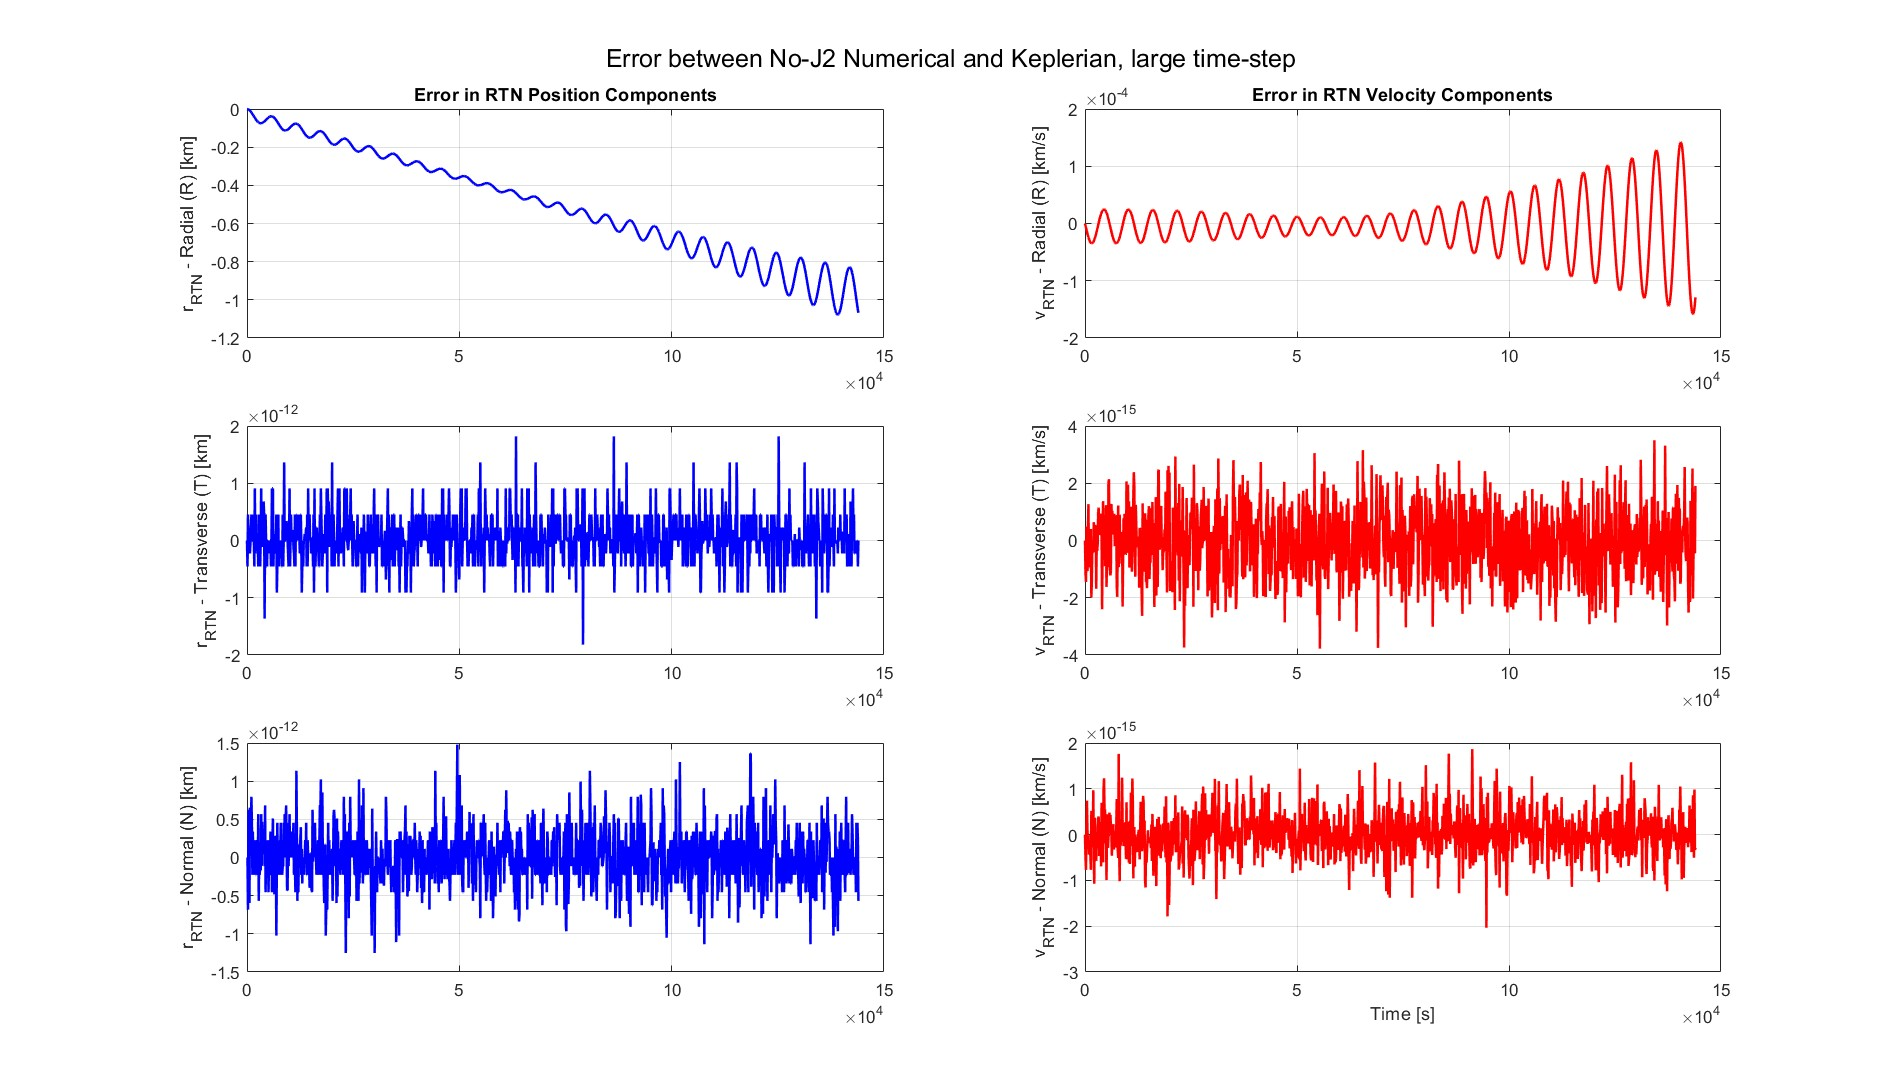
\includegraphics[width=0.75\linewidth]{PS1/Figures/comparing_rtn_large_timestep.jpg}
    \caption{Error in RTN position and velocity, with the large time-step (50 steps per orbit)}
    \label{fig:rtn_compare_large_timestep}
\end{figure}

\begin{figure}[H]
    \centering
    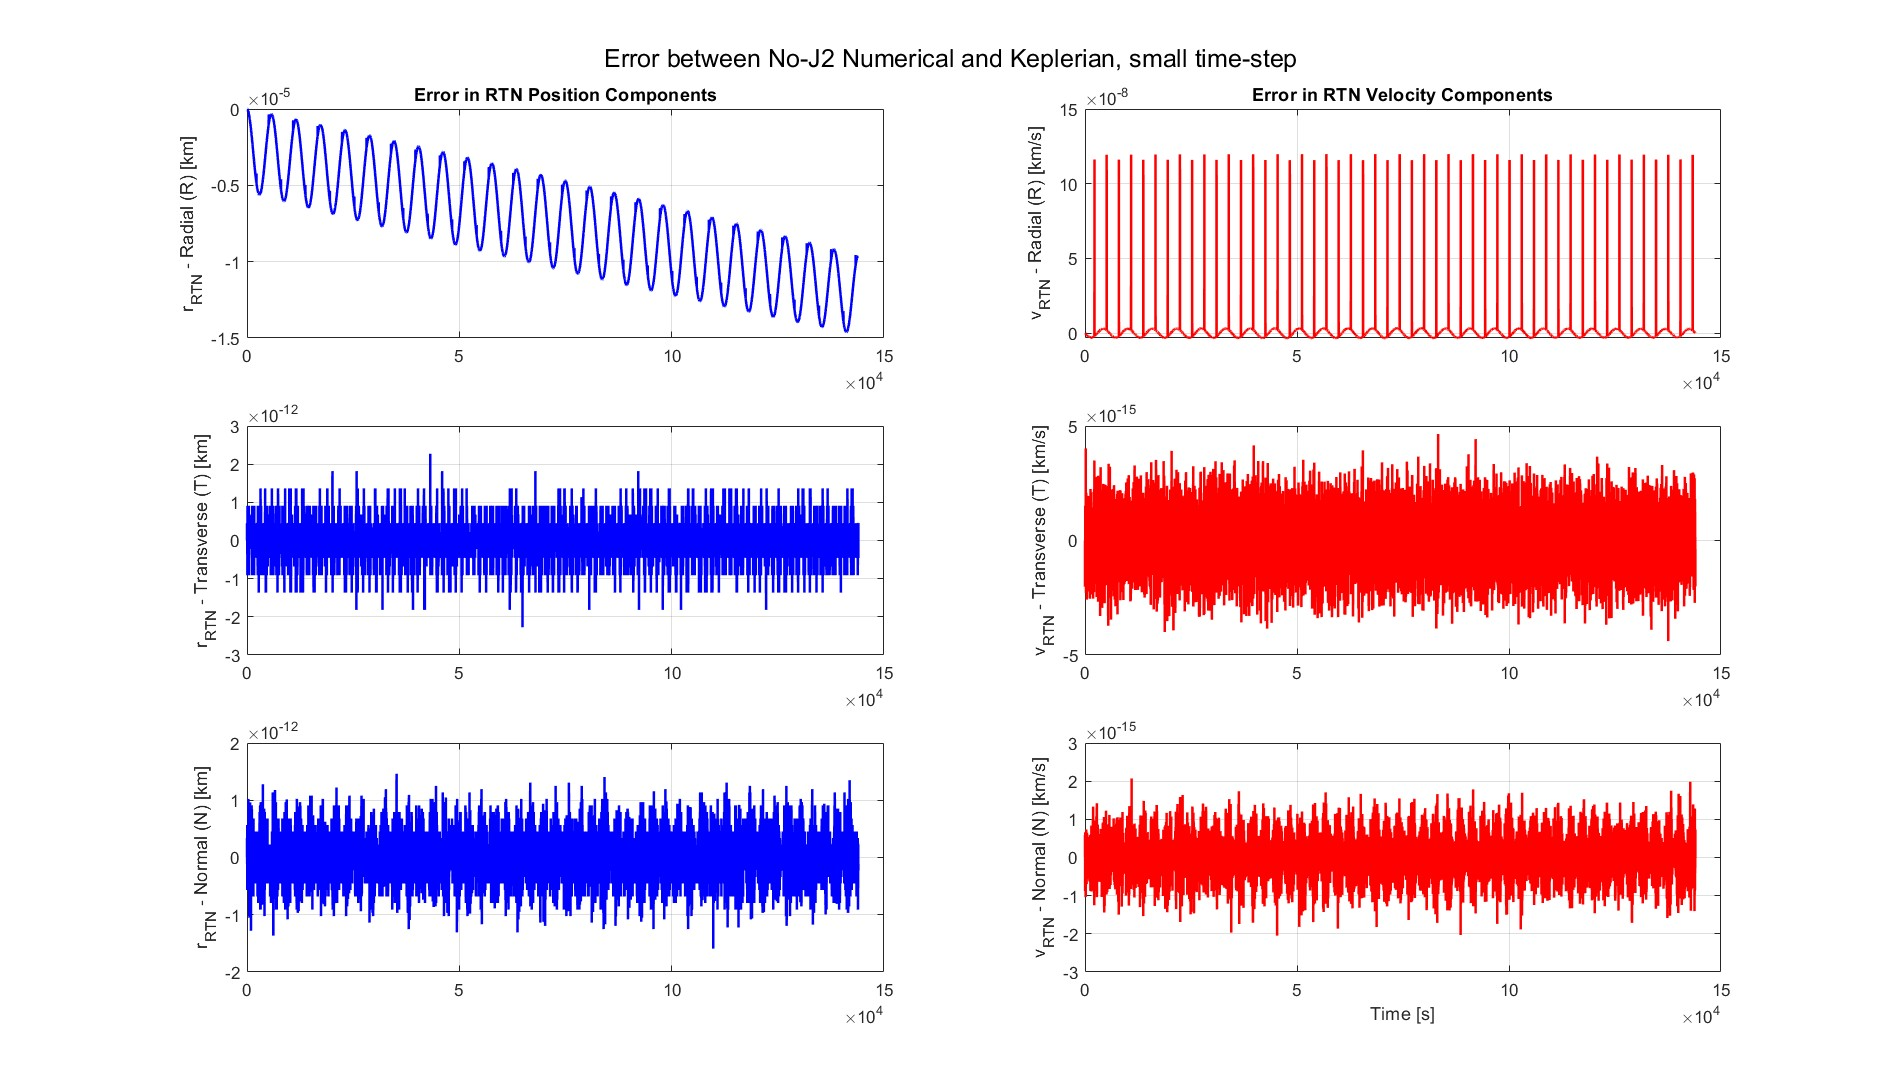
\includegraphics[width=0.75\linewidth]{PS1/Figures/comparing_rtn_small_timestep.jpg}
    \caption{Error in RTN position and velocity, with the small time-step (500 steps per orbit)}
    \label{fig:rtn_compare_small_timestep}
\end{figure}

Based on this, we can conclude that the FODE method that was used here (Fundamental Orbital Differential Equations) starts to accumulate numerical error for larger time-steps. The time-step needs to be reduced to very small values to keep the numerical error from becoming a problem.

\subsubsection{Orbital Elements, Eccentricity Vector, Angular Momentum, Specific Mechanical Energy} \label{sec:oe_compares}

First we compute the osculating Keplerian orbital elements at each time step by converting from the ECI position and velocity at that time step given by our propagator. We then compute the eccentricity vector $\boldsymbol{e}$, the angular momentum vector $\boldsymbol{h}$, and the specific mechanical energy $\epsilon$, throughout the numerical simulations with and without J2 perturbations. To compute these orbital parameters we use the following relationships:

\begin{align}
    \boldsymbol{h} &= \boldsymbol{r}_{ECI} \times \boldsymbol{v}_{ECI} \\
    \boldsymbol{e} &= \frac{\boldsymbol{v}_{ECI} \times \boldsymbol{h}}{\mu_{earth}} - \frac{\boldsymbol{r}_{ECI}}{||\boldsymbol{r}_{ECI}||} \\
    \epsilon &= \frac{||\boldsymbol{v}_{ECI}||^2}{2} - \frac{\mu_{earth}}{||\boldsymbol{r}_{ECI}||}
\end{align}

Figure \ref{fig:j2_oe_comparison} shows the Keplerian orbital elements with and without J2 perturbations over 25 orbits. As expected when excluding J2 effects, all elements remain constant except true anomaly which cycles through 360 degrees. When including J2 effects, we observe periodic and secular effects on all elements, which is expected since J2 acts in all of the RTN directions. The purely periodic effects are seen in semi-major axis, eccentricity, and inclination. The amplitude of these periodic effects are relatively small, especially for inclination and eccentricity. The other three elements - RAAN, argument of periapsis, and true anomaly - experience both periodic and secular drifts, although at different rates of change. This agrees with averaging theory which says that only these three elements experience secular drifts. The largest secular drift is in the RAAN, which is expected from the expressions for average secular drifts. There is also a small but noticeable secular drift in the argument of perigee $\omega$, that also appears in true anomaly. 

\begin{figure}[H]
    \centering
    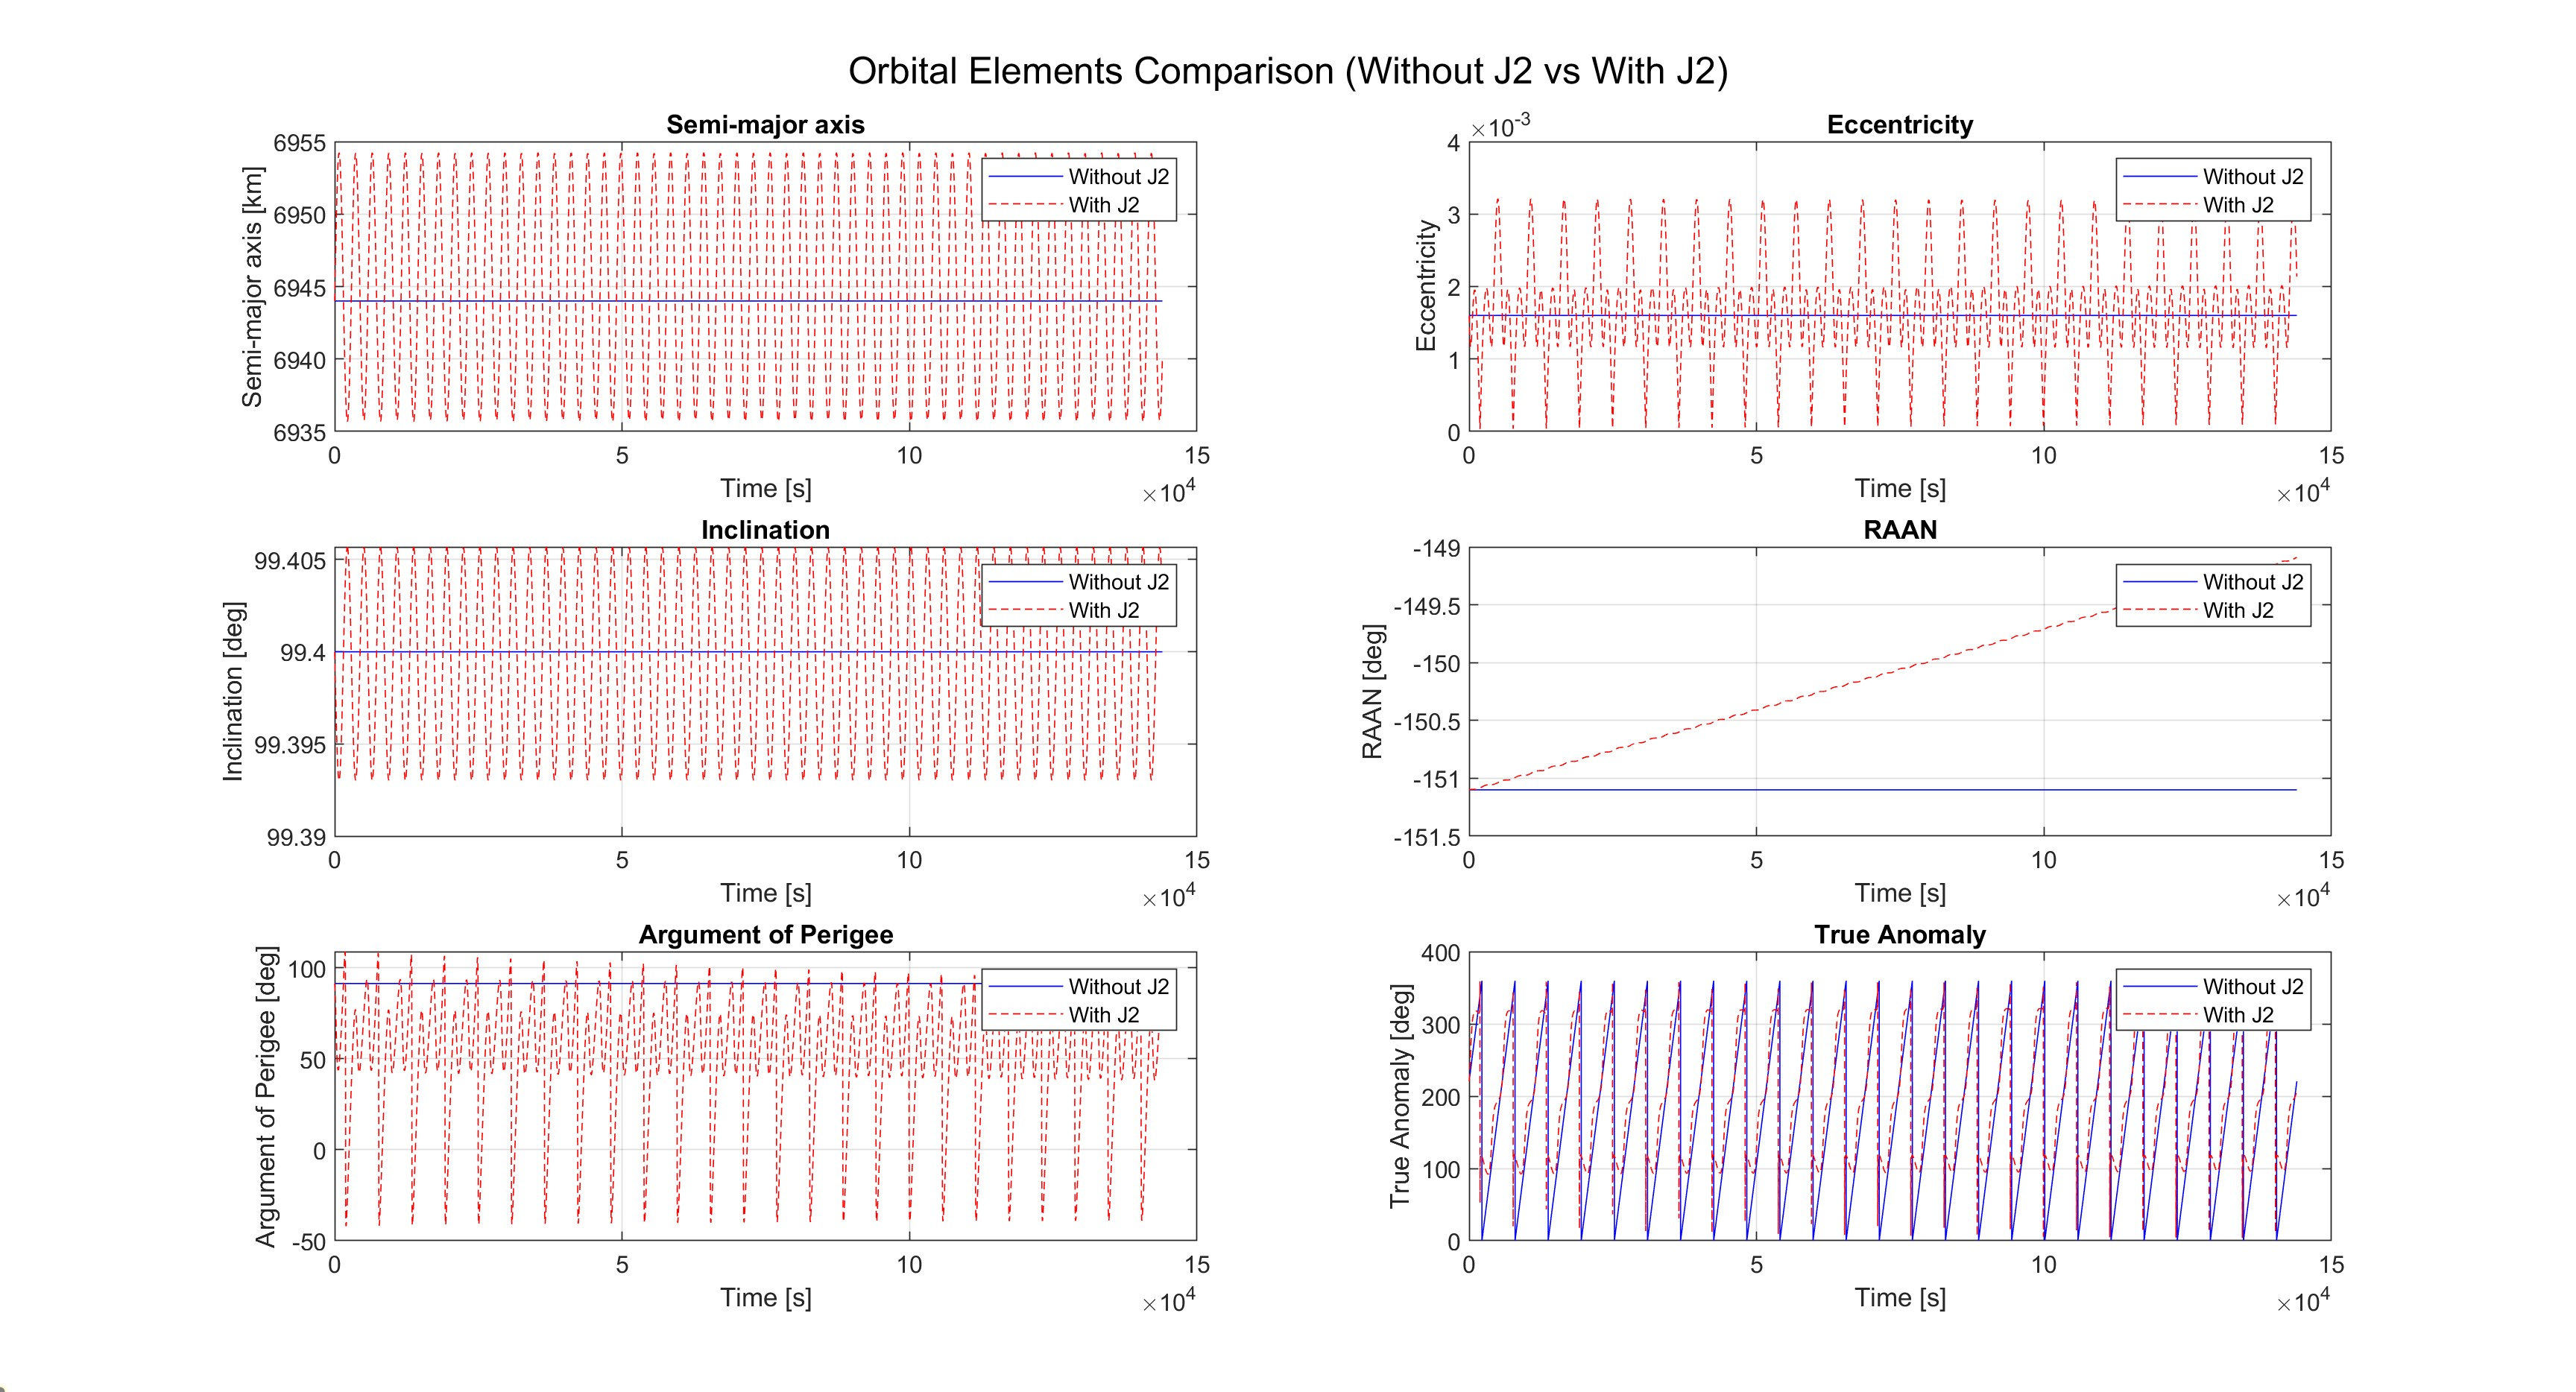
\includegraphics[width=1.1\linewidth]{PS1/Figures/OE_J2_Comparison.jpg}
    \caption{Comparison of Keplerian Orbital Elements with and without J2 perturbations over 25 orbits}
    \label{fig:j2_oe_comparison}
\end{figure}

\begin{figure}[H]
    \centering
    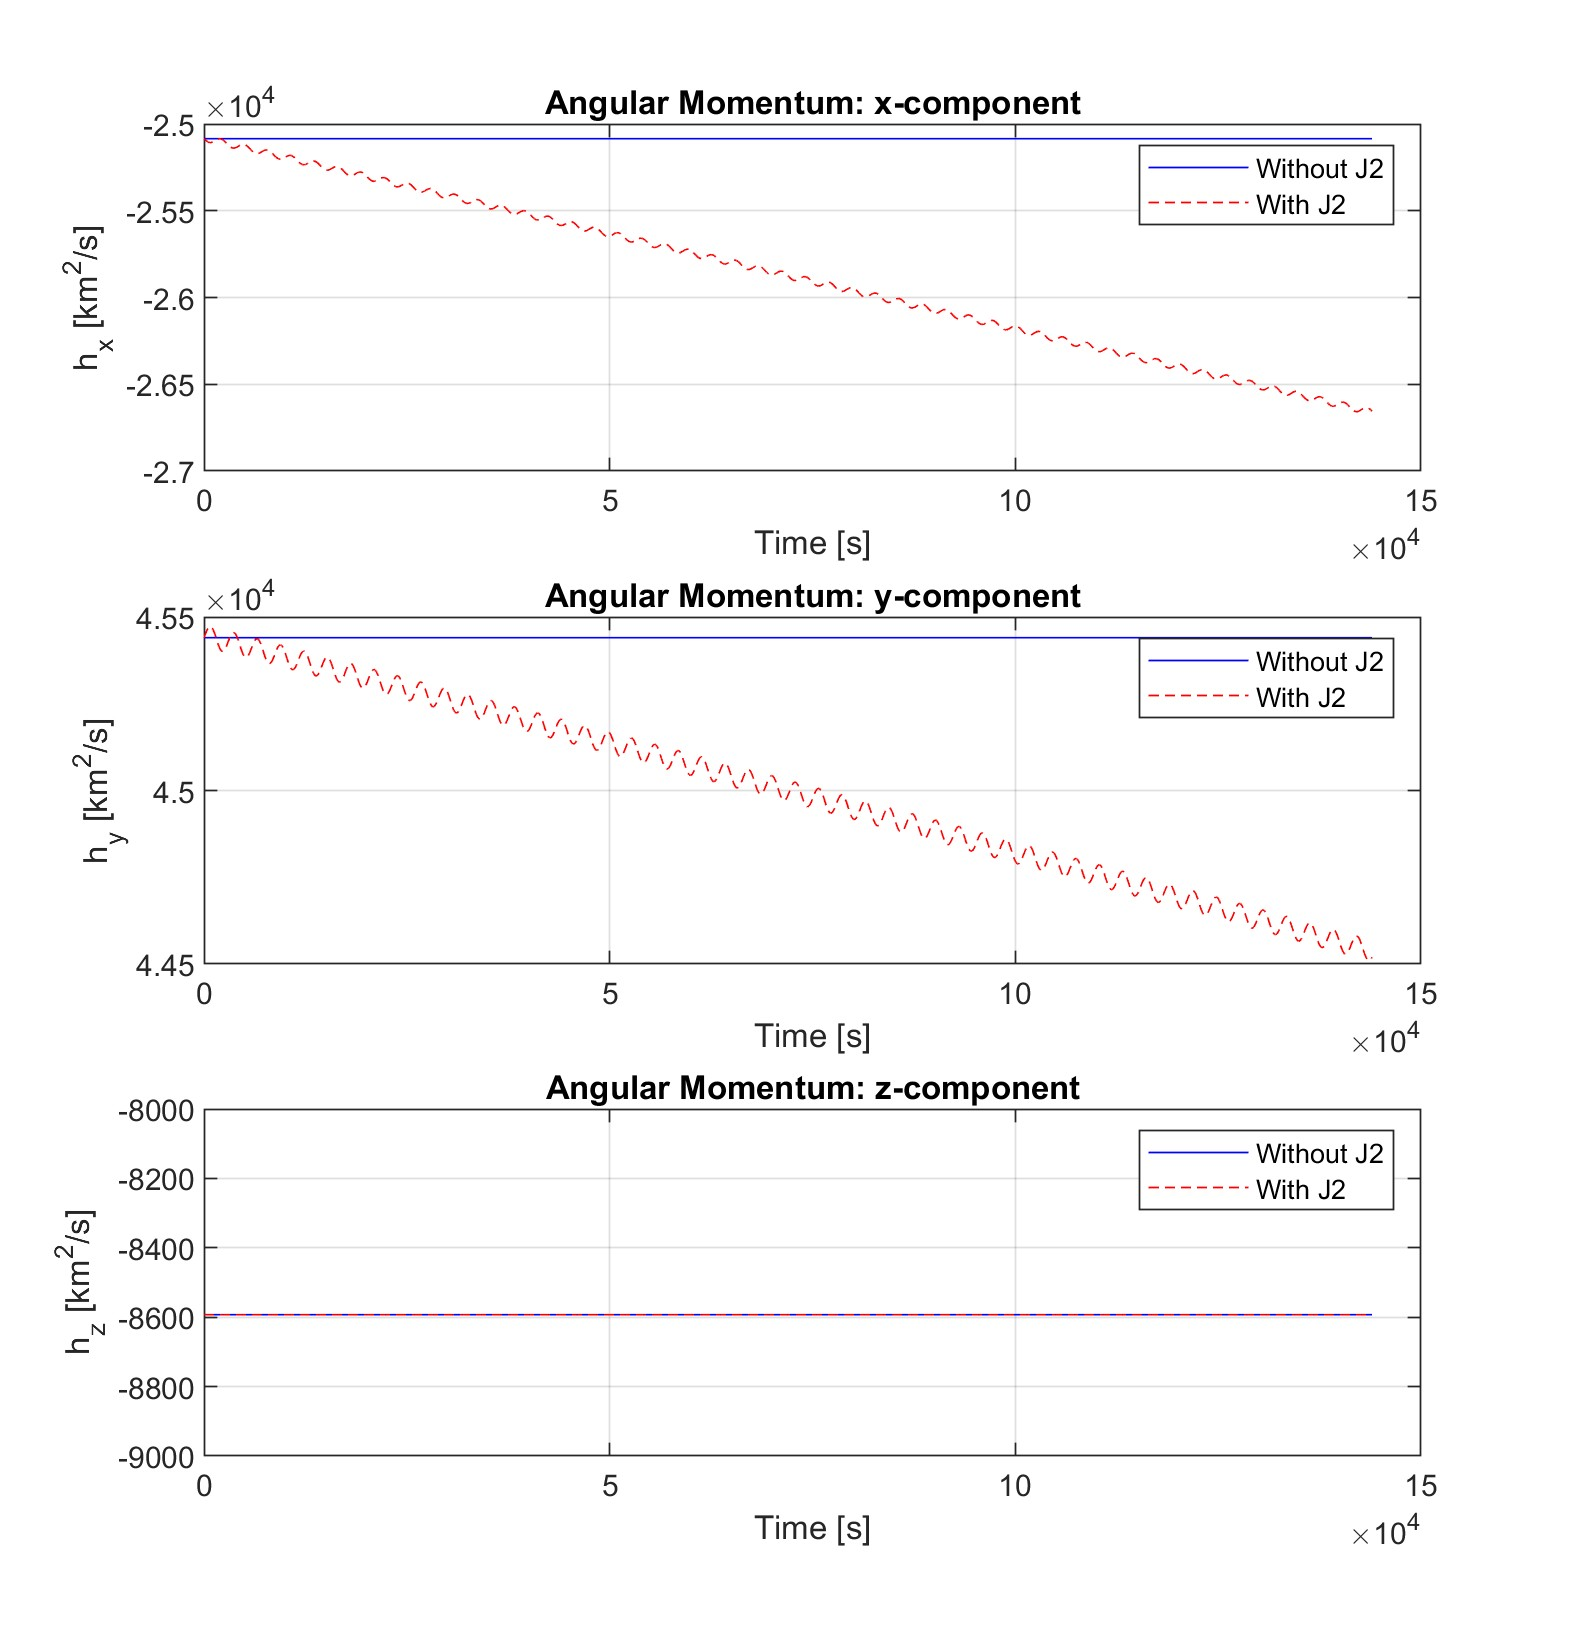
\includegraphics[width=0.5\linewidth]{PS1/Figures/h_J2_comparison.jpg}
    \caption{Comparison of Angular Momentum Vector with and without J2 perturbations over 25 orbits}
    \label{fig:angular_momentum}
\end{figure}

Figure \ref{fig:angular_momentum} compares the angular momentum vector over 25 orbits with and without J2. As expected without J2, the angular momentum vector remains constant. As expected from averaging theory, with J2 there are secular drifts in the x and y components of angular momentum. The z component remains constant because the angular velocity vector is tracing out a cone due to the effects of J2. There are also short-periodic effects on these components from J2.  

\begin{figure}[H]
    \centering
    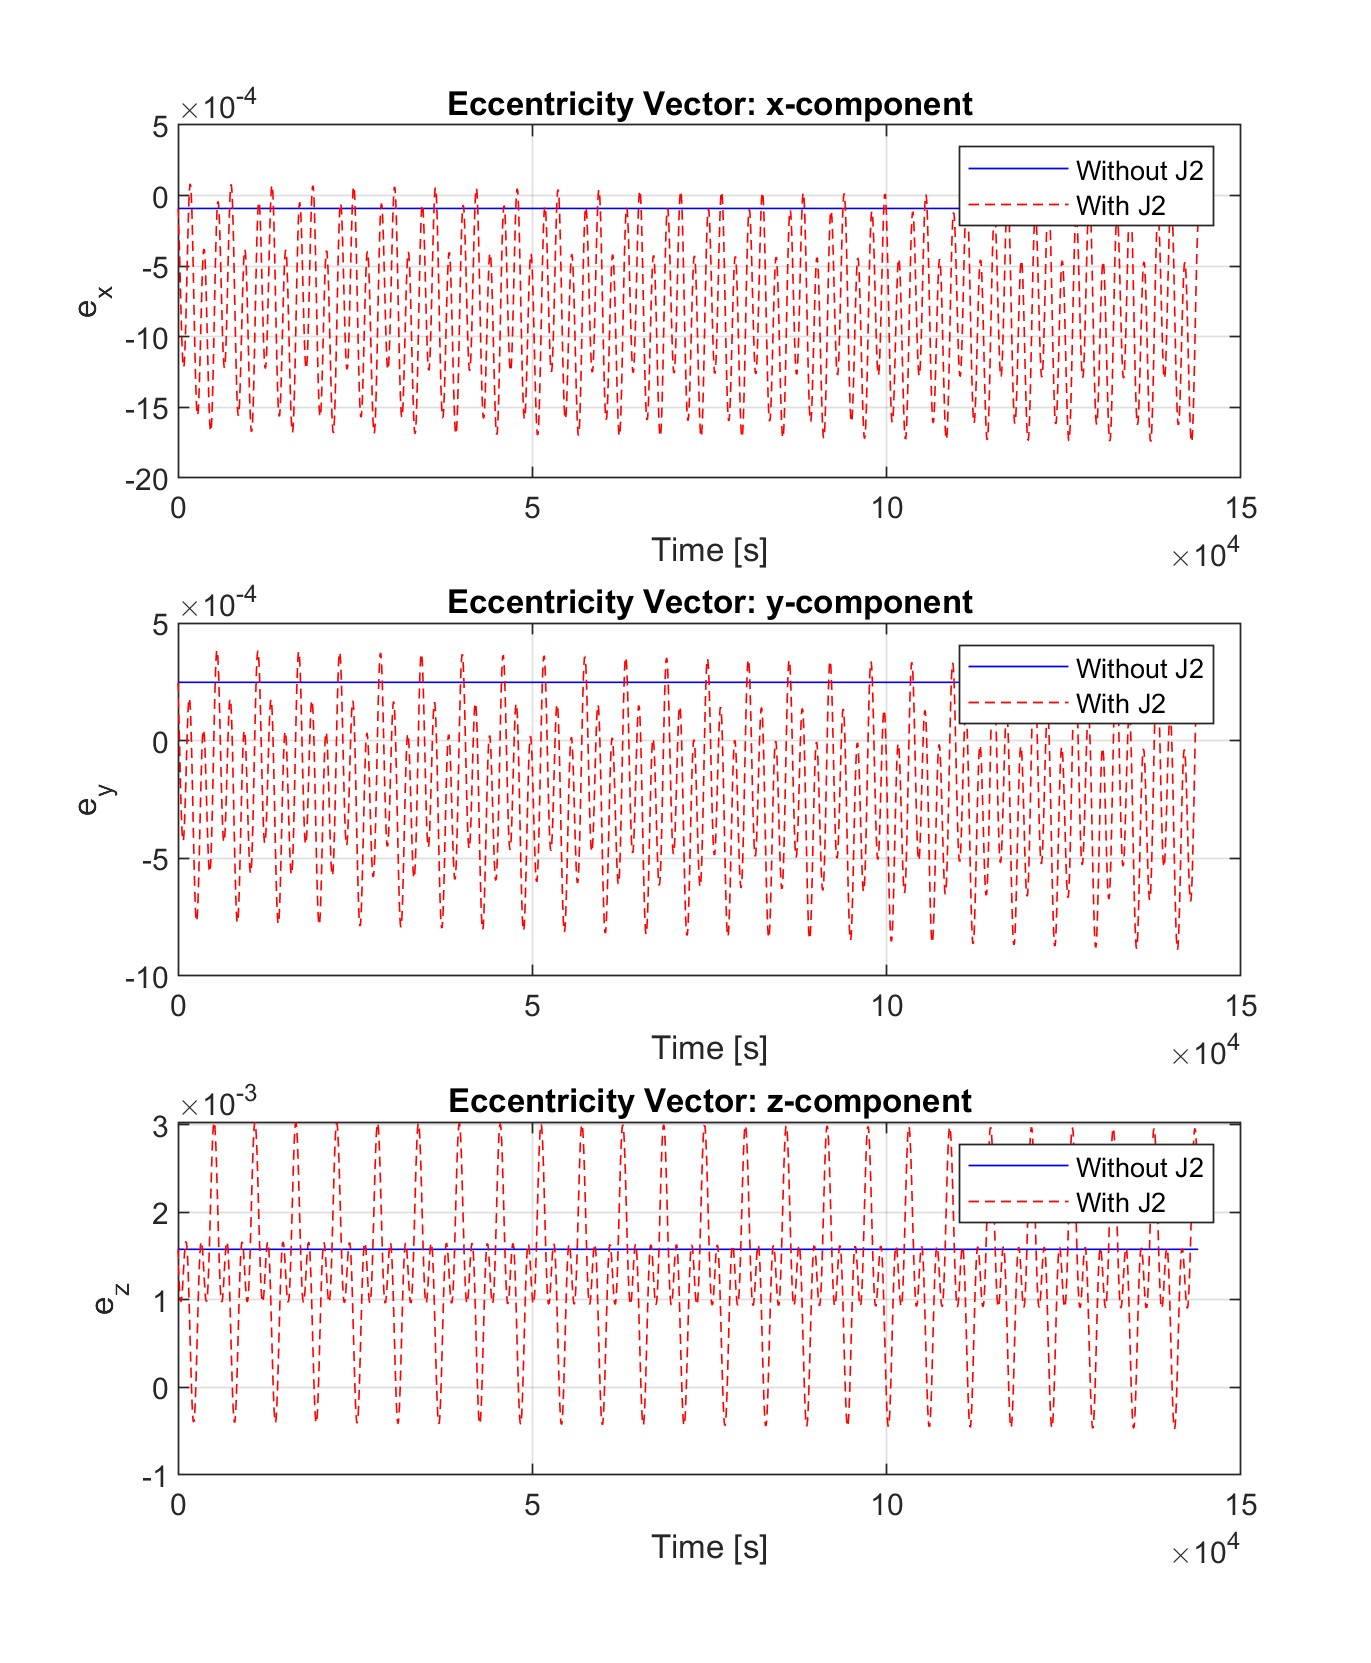
\includegraphics[width=0.5\linewidth]{PS1/Figures/ecc_J2_comparison.jpg}
    \caption{Comparison of Eccentricity Vector with and without J2 perturbations over 25 orbits}
    \label{fig:eccentricity_vector}
\end{figure}

Figure \ref{fig:eccentricity_vector} compares the eccentricity vector over 25 orbits with and without J2. As expected, without J2, the eccentricity vector remains constant. As expected from averaging theory, with J2 there are secular drifts in the x and y components of the eccentricity vector. This corresponds to the secular drift in the argument of periapsis. There are also short-periodic effects on these components from J2.  


Figure \ref{fig:specific_energy} compares the specific mechanical energy over 25 orbits with and without J2. As expected, without J2, the specific mechanical energy remains constant. With J2, the average specific mechanical energy also remains constant, which is expected since gravity is a conservative force and thus will not affect the specific mechanical energy. The periodic behavior with J2 may be due to computational error. 

\begin{figure}[H]
    \centering
    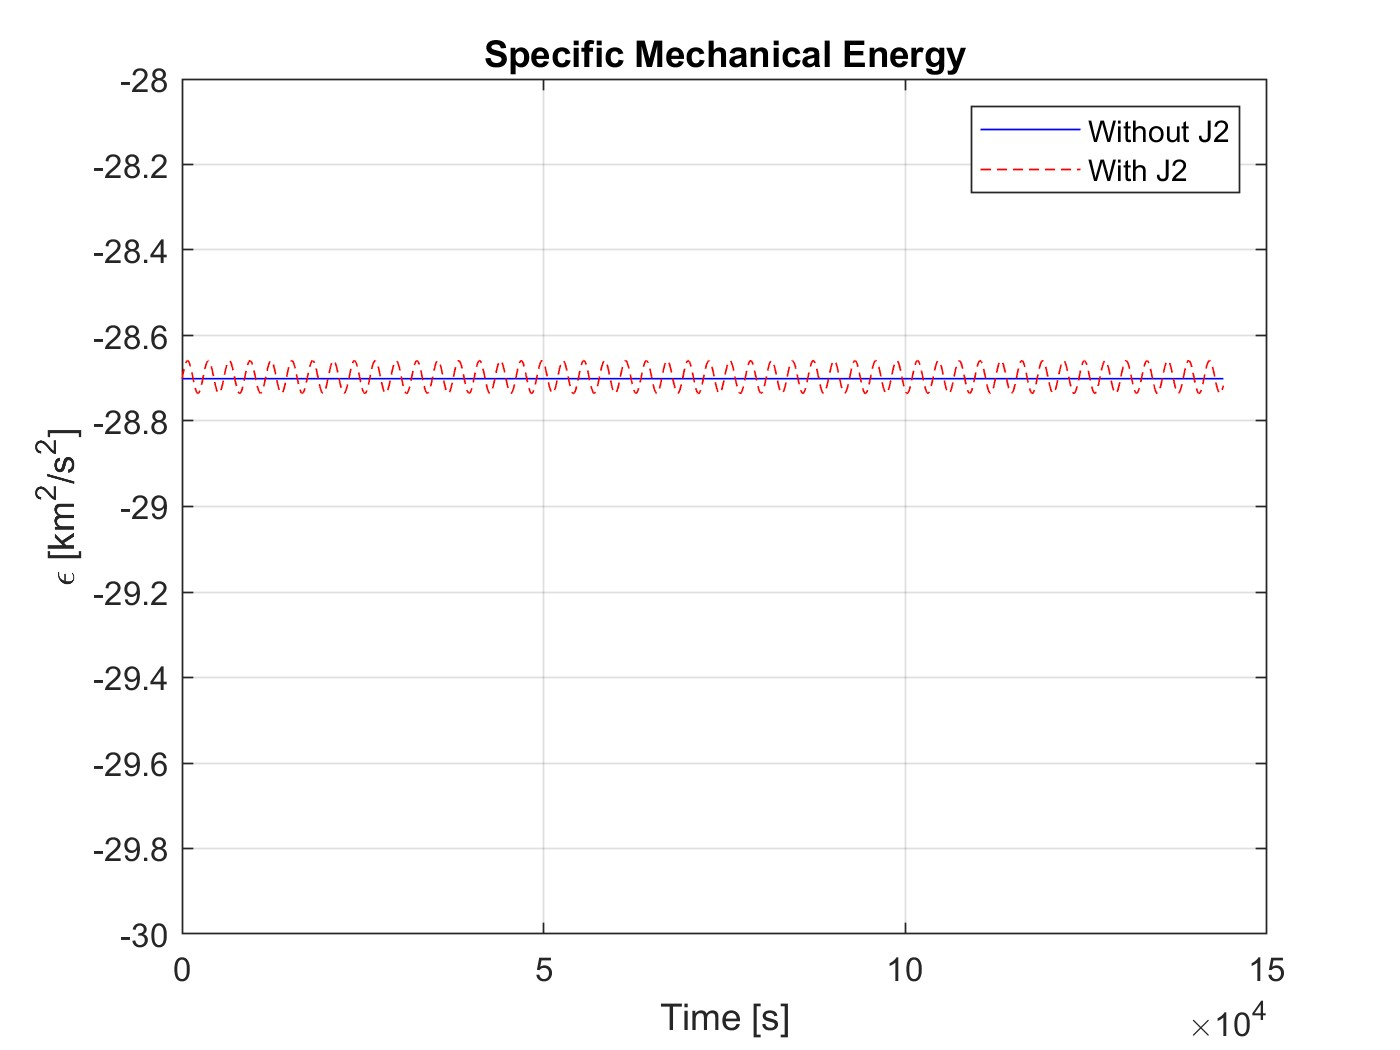
\includegraphics[width=0.5\linewidth]{PS1/Figures/Epsilon_J2_Comparison.jpg}
    \caption{Comparison of Specific Mechanical Energy with and without J2 perturbations over 25 orbits}
    \label{fig:specific_energy}
\end{figure}

\subsubsection{Osculating vs. Mean Orbital Elements with J2 Comparison}
Now, to compare these results with the secular Gauss Variational Equations for J2 with mean orbital elements, we numerically integrate the following linear differential equations:
\begin{align}
\frac{d e_x}{dt} &= -\frac{3}{4} n J_2 \left( \frac{R_\oplus}{a \left(1 - (e_x^2 + e_y^2)\right)} \right)^2 e_y (5 \cos^2 i - 1) \\
\frac{d e_y}{dt} &= \phantom{-}\frac{3}{4} n J_2 \left( \frac{R_\oplus}{a \left(1 - (e_x^2 + e_y^2)\right)} \right)^2 e_x (5 \cos^2 i - 1) \\
\frac{d\Omega}{dt} &= -\frac{3}{2} n J_2 \left( \frac{R_\oplus}{a \left(1 - (e_x^2 + e_y^2)\right)} \right)^2 \cos i  \\
\frac{du}{dt} &= \frac{3}{4} n J_2 \left( \frac{R_\oplus}{a \left(1 - (e_x^2 + e_y^2)\right)} \right)^2 
\left[ \sqrt{1 - (e_x^2 + e_y^2)} (3 \cos^2 i - 1) + (5 \cos^2 i - 1) \right] \quad 
\end{align}

Figure \ref{fig:osc_mean_oe} superimposes the resulting mean and osculating orbital elements on top of each other. As expected, the mean semi-major axis, eccentricity, and inclination remain constant even with J2. For these elements, the osculating elements are purely periodic, agreeing with the mean ones. For RAAN, there both mean and osculating exhibit a clear secular growth. For both argument of periapsis and true anomaly, the osculating elements exhibit periodic and secular behavior. The secular drift in both lines up with the secular drift seen in the mean elements.

\begin{figure}[H]
    \centering
    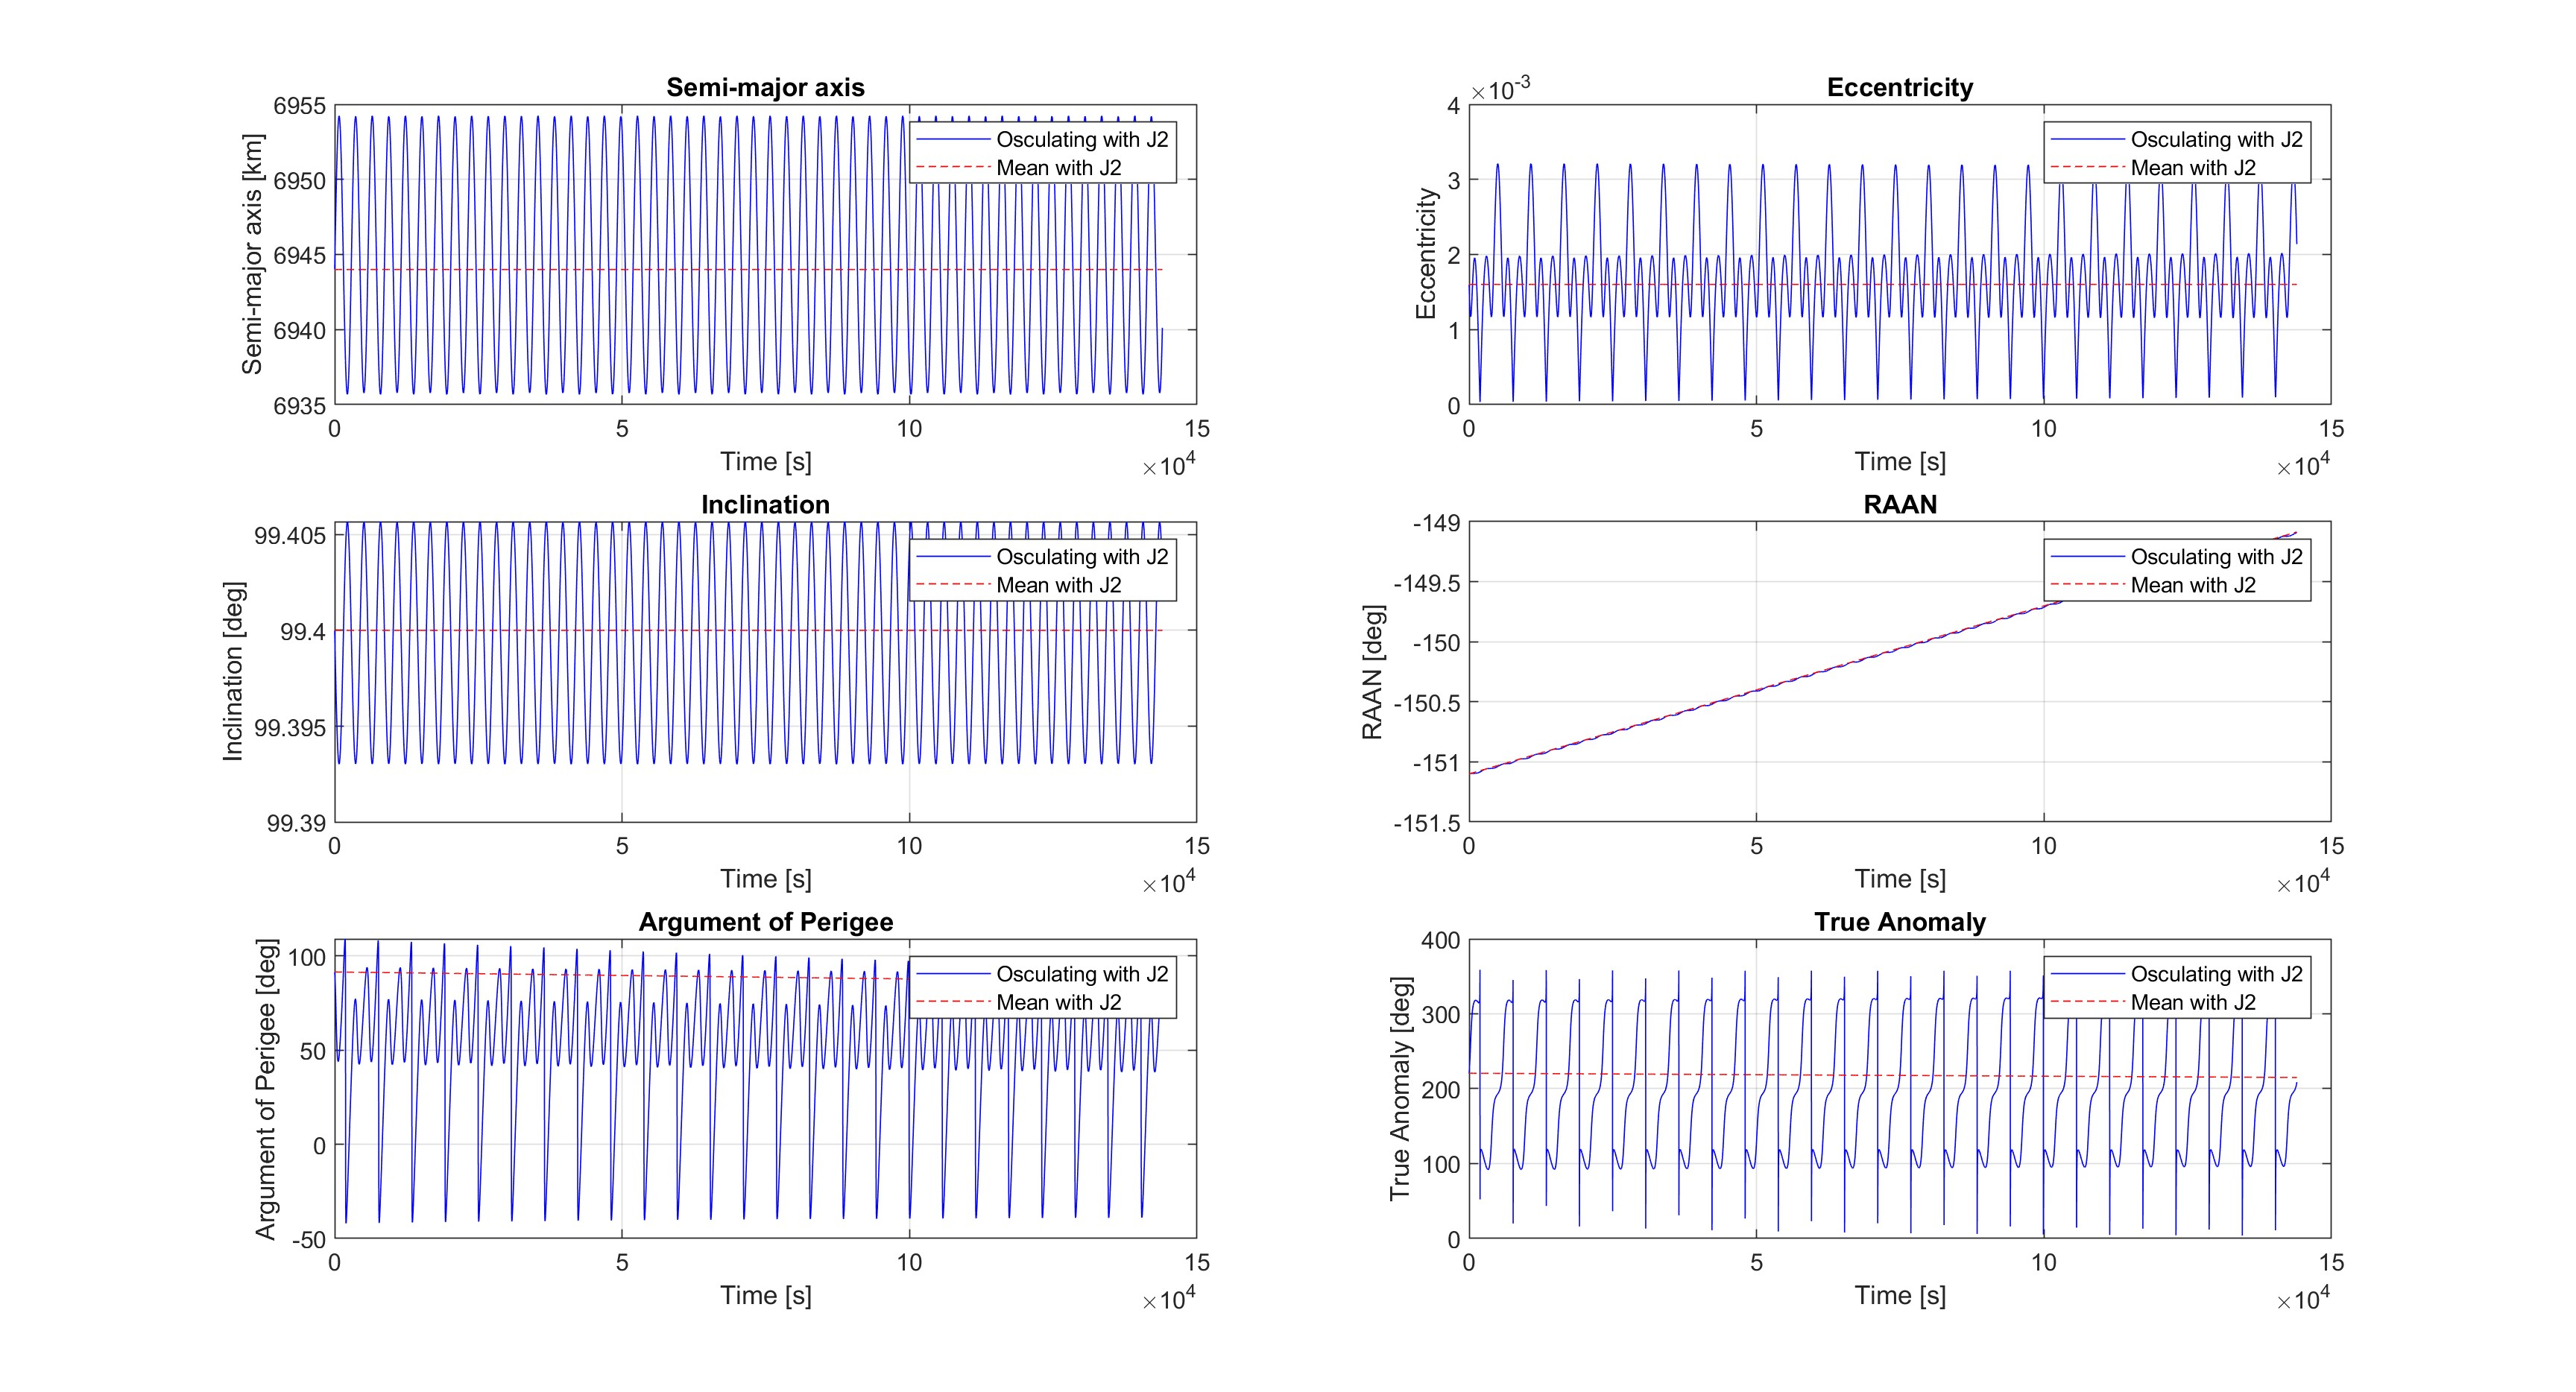
\includegraphics[width=1.1\linewidth]{PS1/Figures/OE_mean_osc_J2_comparison.jpg}
    \caption{Osculating vs Mean Orbital Elements with J2}
    \label{fig:osc_mean_oe}
\end{figure}

\subsubsection{Issues with Comparison}
Issues could arise from the comparison of osculating and mean orbital elements due to the initialization procedure. Specifically, we interpreted our initial orbital elements as osculating at first and then as mean states later on. To ensure that the comparisons remain consistent, it would be most appropriate to convert our initial orbital elements from mean to osculating at first. Furthermore, to ensure that both methods align, the final results from osculating could be converted to mean elements to numerically determine if there are any discrepancies, rather than by visual inspection.
